\subsection{Preparação do ambiente}

\par Visto que o trabalho seria desenvolvido em equipe, foi necessário estabelecer uma ferramenta de controle de versão. Esta ferramente permitiu o gerenciamento de diferentes versões de arquivos, mantendo um histórico com as modificações que foram realizadas no decorrer do processo de desenvolvimento. Este histórico permite o retorno de alguma revisão, caso haja necessidade. A ferramenta escolhida para realizar esse controle foi o GitHub, que já havia sido utilizado em alguns trabalhos do contexto acadêmico, evitando o desprendimento de tempo para estudo de uma nova ferramenta de apoio. O GitHub é uma ferramenta bem difundida e permite que os seus usuários colaborem com os projetos que estão armazenados em seus repositórios\footnotemark[31]. A Figura~\ref{fig:github_inicio} demonstra a tela de serviços provida pelo GitHub.

\footnotetext[31]{Repositório: local cujo desenvolvedor utiliza para armazenar os documentos relacionados ao \textit{software}.}

\begin{figure}[h!]
	\centerline{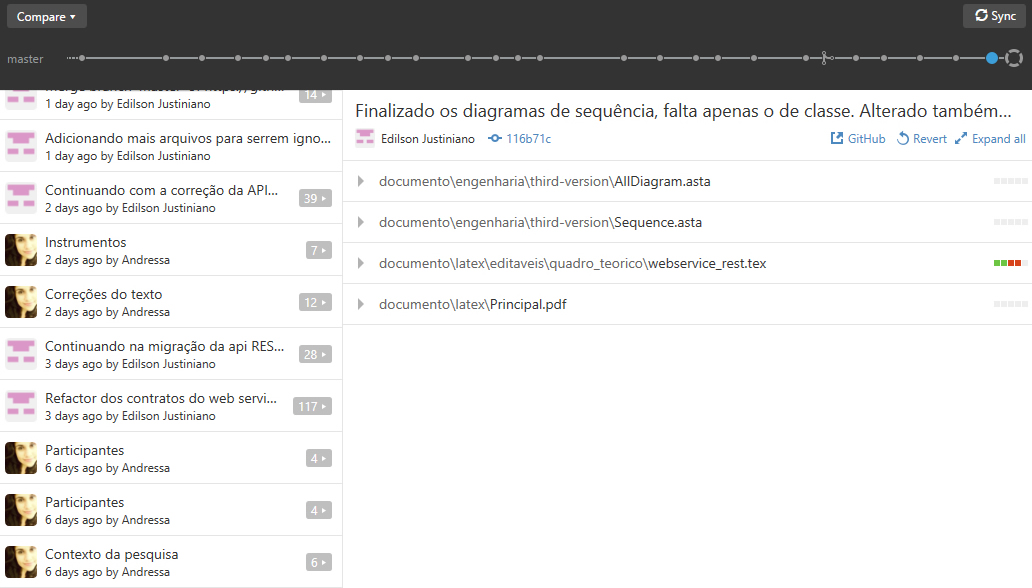
\includegraphics[scale=0.3]{./imagens/github.jpg}}
	\caption[Tela de serviços do GitHub ]
	{Tela de serviços do GitHub \textbf{Fonte:} Elaborado pelos autores.}
	\label{fig:github_inicio}
\end{figure}

\par Os passos de instalação detalhados do GitHub são descritos  no Apêndice I deste trabalho.

\par Como mencionado no quadro teórico, neste trabalho foi utilizada a linguagem Java, sendo assim necessária a utilização de uma \textit{Integrated Development Environment} - IDE\footnotemark[32] - de apoio. A IDE escolhida foi o Eclipse, pois se trata de uma ferramenta \textit{open source}, muito utilizada no mercado e que permite a escrita de um código mais legível, facilitando tarefas como \textit{debug} e configurações do trabalho.

\footnotetext[32]{IDE: \textit{Integrated Development Environment} - Aplicação contendo uma série de ferramentas para auxiliar no desenvolvimento de \textit{software}.}

\par O Eclipse possui várias ferramentas, dentre elas, pode-se citar o editor de texto, usado não somente para a escrita de códigos em Java, e também a perspectiva de configuração para servidores \textit{web}, utilizada neste trabalho, conforme apresenta a Figura~\ref{fig:ide_eclipse}. Por meio desta perspectiva, foi configurada a aplicação \textit{container} Tomcat na versão 7.

\begin{figure}[h!]
	\centerline{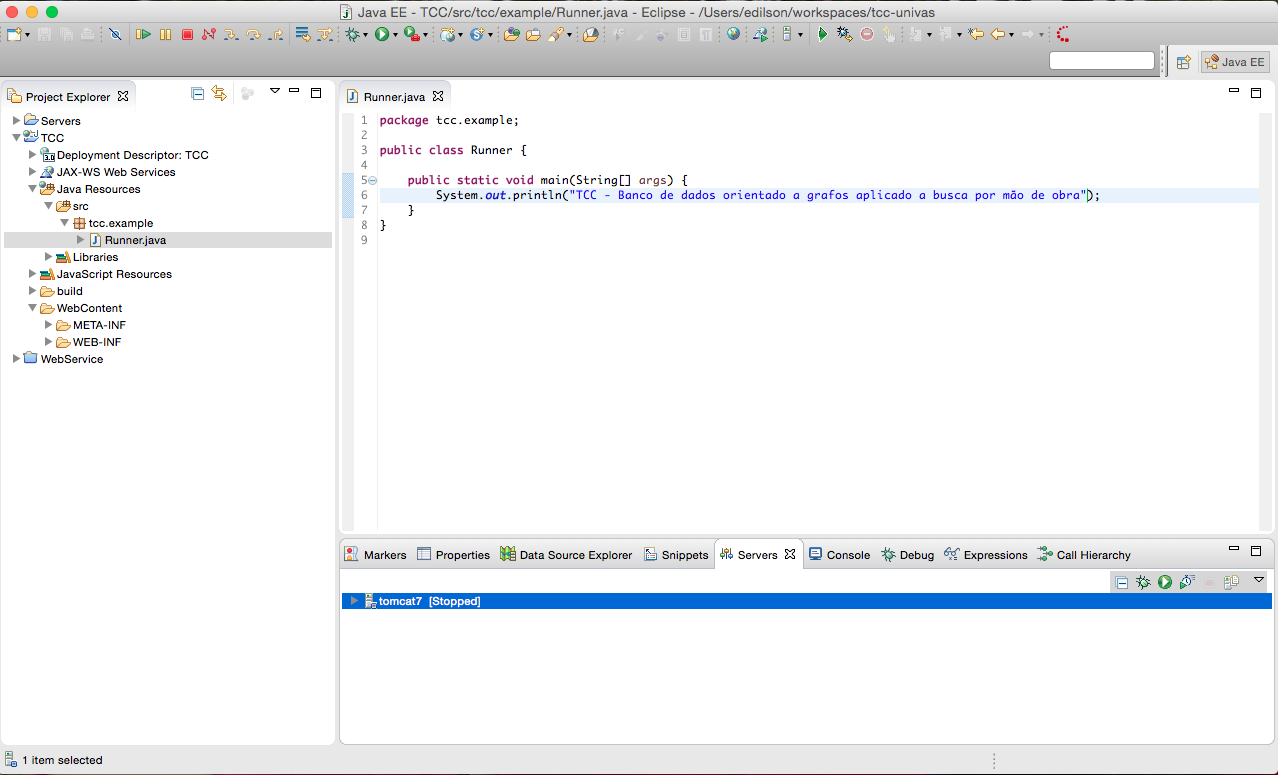
\includegraphics[scale=0.3]{./imagens/eclipse-editor-texto.png}}
	\caption[Ferramentas da IDE Eclipse]
	{Ferramentas da IDE Eclipse \textbf{Fonte:} Elaborado pelos autores.}
	\label{fig:ide_eclipse}
\end{figure}

\par O Tomcat desempenhou um papel fundamental na execução desta aplicação, pois serviu como hospedeiro para a aplicação Java desenvolvida neste trabalho. 

\par Os passos de instalação e configuração do Eclipse e do Tomcat são descritos no Apêndice II deste trabalho.

\par Para a escrita do código relacionado ao HTML, CSS e Javascript, foi utilizado o mesmo editor de texto citado anteriormente.

\par O trabalho fez uso de um banco de dados orientado a grafos, o Neo4j. A escolha desse banco se deu pela sua simplicidade de instalação, configuração, facilidade de integração com a API \textit{Cypher} e por disponibilizar uma API REST para acesso aos seus dados, conforme descrito no quadro teórico deste trabalho. O Neo4j faz parte do enquadramento de softwares livres, seguindo o conceito \textit{open source}, o que permite ao desenvolvedor utilizá-lo da forma que melhor lhe convier. 

\par Os passos para a instalação do banco de dados Neo4j são detalhados no Apêndice III deste trabalho.

\par Posterior à configuração do ambiente, iniciou-se o desenvolvimento propriamente dito, apresentado a seguir.
